\renewcommand{\theequation}{\theenumi}
\begin{enumerate}[label=\arabic*.,ref=\thesubsubsection.\theenumi]
\numberwithin{equation}{enumi}

\item In the given question,
\\
The sample size = Possible number of tosses=8
\begin{align}
\resizebox{\columnwidth}{!}{%
\myvec{\bmat{HHH}&\bmat{TTT}&\bmat{HHT}&\bmat{HTT}&\bmat{HTH}&\bmat{TTH}\bmat{THT}&\bmat{THH}}
}
\end{align}
Favourable outcome =Other than three Heads (or) Tails=6
\begin{align}
\resizebox{\columnwidth}{!}{%
\myvec{\bmat{HHT}&\bmat{HTT}&\bmat{HTH}&\bmat{TTH}\bmat{THT}&\bmat{THH}}
}
\end{align}
Probabilty(P) that Hanif will loose the game=$\frac{6}{8}$
\\
$\therefore$ P = 0.75
\label{eq:prob}
\\
The python code for the figure \ref{fig:figure}
\begin{lstlisting}
prob/codes/prob4.py
\end{lstlisting}
shows the Bernouli distribution of data.
\begin{figure}[!ht]
\centering
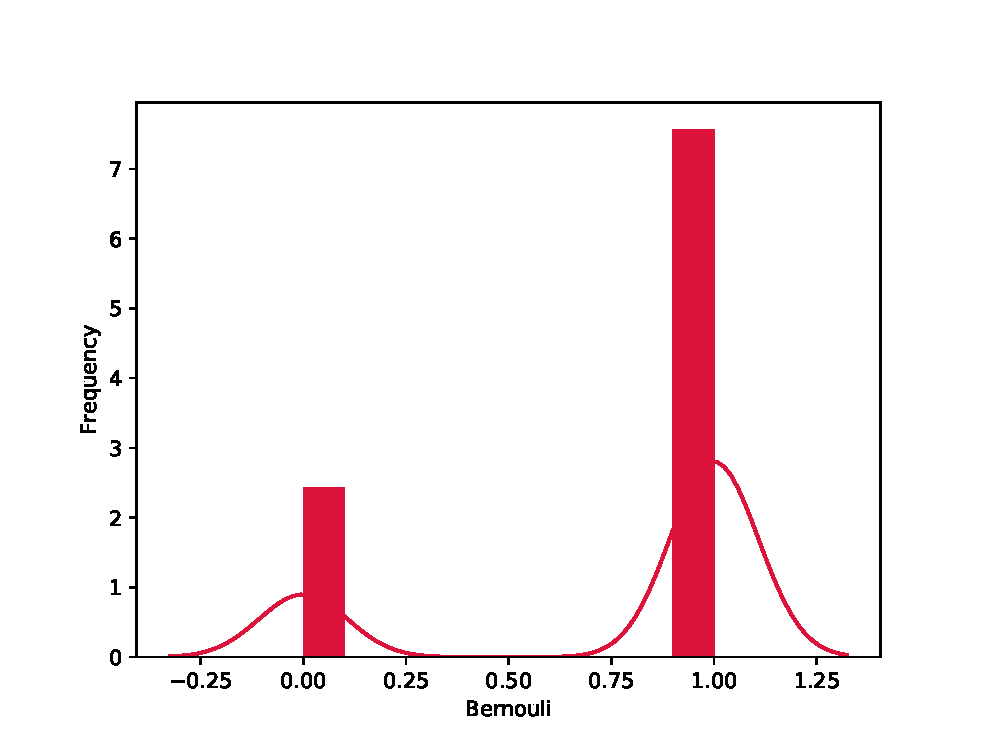
\includegraphics[width=\columnwidth]{./prob/figs/prob4.eps}
\caption{Bernoulli Distribution.}
\label{fig:figure}
\end{figure}
\\
The Bernoulli Distribution of data is given below
\\
Probability mass function(P(X))=$p^x\brak{1-p}^{1-x}$
\begin{align}
P(X=0)=1-p
\\
P(X=1)=p
\end{align}
where p=0.75 given by \ref{eq:prob}
\end{enumerate}